\section{Ocaml Basics: Syntax, Types, and Semantics}

\subsection*{Strong Typing}

OCaml is a strongly typed language, meaning that operations between incompatible types are not allowed. Additionally, the underscore (\texttt{\_}) is used as a throwaway variable for values that are not intended to be used.

\begin{lstlisting}[language=OCaml, caption={Example of Strong Typing}]
    let x : int = 2
    let y : string = "two"
    let _ = x + y (* THIS IS NOT POSSIBLE *)
\end{lstlisting}

\noindent
This will result in the following error:
\begin{lstlisting}[language=Bash, caption={Error Message}]
    3 | let _ = x + y (* THIS IS NOT POSSIBLE *)
        ^ 
    Error: This expression has type string but an expression was expected of type int
\end{lstlisting}

\noindent
Demonstrating that, in OCaml, unlike other languages, operator overloading and implicit type conversions are not allowed.
This means, no adding strings and integers, floats and integers, etc. There are separate operators for each type.\\

\noindent
\textbf{Basic Ocaml Operators:}\\
Operators in OCaml behave just like other languages, with a few exceptions. Here are the basic operators at a quick
glance:

\vspace{.5em}
\begin{table}[h!]
    \centering
    \resizebox{\textwidth}{!}{%
    \begin{tabular}{|c|c|c|}
    \hline
    \rowcolor{OliveGreen!10}\textbf{Type}   & \textbf{Literals Examples}             & \textbf{Operators}           \\ \hline
    \texttt{int}    & \texttt{0, -2, 13, -023}      & \texttt{\textcolor{Wine}{+}, \textcolor{Wine}{-}, \textcolor{Wine}{*}, \textcolor{Wine}{/}, \textcolor{Wine}{mod}}      \\ \hline
    \texttt{float}  & \texttt{3., -1.01}            & \texttt{\textcolor{Wine}{+.}, \textcolor{Wine}{-.}, \textcolor{Wine}{*.}, \textcolor{Wine}{/.}}       \\ \hline
    \texttt{bool}   & \texttt{true, false}          & \texttt{\textcolor{Wine}{\&\&}, \textcolor{Wine}{||}, \textcolor{Wine}{not}}        \\ \hline
    \texttt{char}   & \texttt{'b', 'c'}             &                               \\ \hline
    \texttt{string} & \texttt{"word", "@*\&\#"}     & \textcolor{Wine}{$^\wedge$}                  \\ \hline
    \end{tabular}%
    }
    \caption{Basic OCaml Types, Literals, and Operators}
    \label{tab:ocaml-types}
\end{table}

\newpage 

\noindent
For emphasis:
\begin{Def}[OCaml Operators]

    \noindent
    \textbf{Operator Distinctions:}\\
    Operators for \snippet{int} and \snippet{float} are \textit{different}. For example:
    \begin{itemize}
        \item \snippet{+} (integer addition)
        \item \snippet{+.} (float addition)
        \item \snippet{$^\wedge$} (string concatenation)
    \end{itemize}
    
    \noindent
    Moreover, the \snippet{mod} operator is used for integer division. This is to 
    say that there is no implicit type conversion in OCaml.\\
    \rule{\textwidth}{0.4pt}

    \vspace{.3em}
    \noindent
    \textbf{No Operator Overloading:}\\
    OCaml has \underline{\textbf{no operator overloading}}, meaning operators are strictly tied to specific types.

    \vspace{.3em}
    \noindent
    \rule{\textwidth}{0.4pt}

    \vspace{.3em}
    \noindent
    \textbf{Comparison Operators:}\\
    Comparison operators are standard and can be used to compare expressions of the same type:
    \begin{itemize}
        \item \snippet{<}, \snippet{<=}, \snippet{>}, \snippet{>=}
    \end{itemize}

    \vspace{-.3em}
    \noindent
    \rule{\textwidth}{0.4pt}
    
    \noindent
    \textbf{Equality and Inequality:}

    \vspace{-.5em}
    \begin{itemize}
        \item Equality check: \snippet{=}
        \item Inequality check: is \snippet{<>} \textbf{and not}, \snippet{!=}
    \end{itemize}

    \vspace{-1em}
    
\end{Def}

\vspace{-1em}
\noindent
\begin{Def}[OCaml (in) Keyword]
    
Consider the expression below:
\begin{lstlisting}[language=OCaml, numbers=none]
    let x = 2 in x + x 
\end{lstlisting}

\noindent
The \snippet{in} keyword is used to bind the value of \snippet{x} to the expression \snippet{x + x}. This is a common pattern in OCaml.
In a sense we are saying, `` let $x$ stand for 2 in the expression $x + x$.''\\

This is similar to the prerequisite definition of the substitution operation (\ref{def:substitution}). Mathematically, we can think of this as:
\[
    [2/x](x + x) = 2 + 2
\]

\noindent
Where the value of 2 is substituted for $x$ in the expression $x + x$.

\end{Def}
\newpage 

\noindent
To illustrate this, Observe the diagram below:\\

\vspace{-1em}

\begin{figure}[h]
    {
    \setlength{\fboxsep}{10pt}
    \centering
    \fbox{\hspace{2em}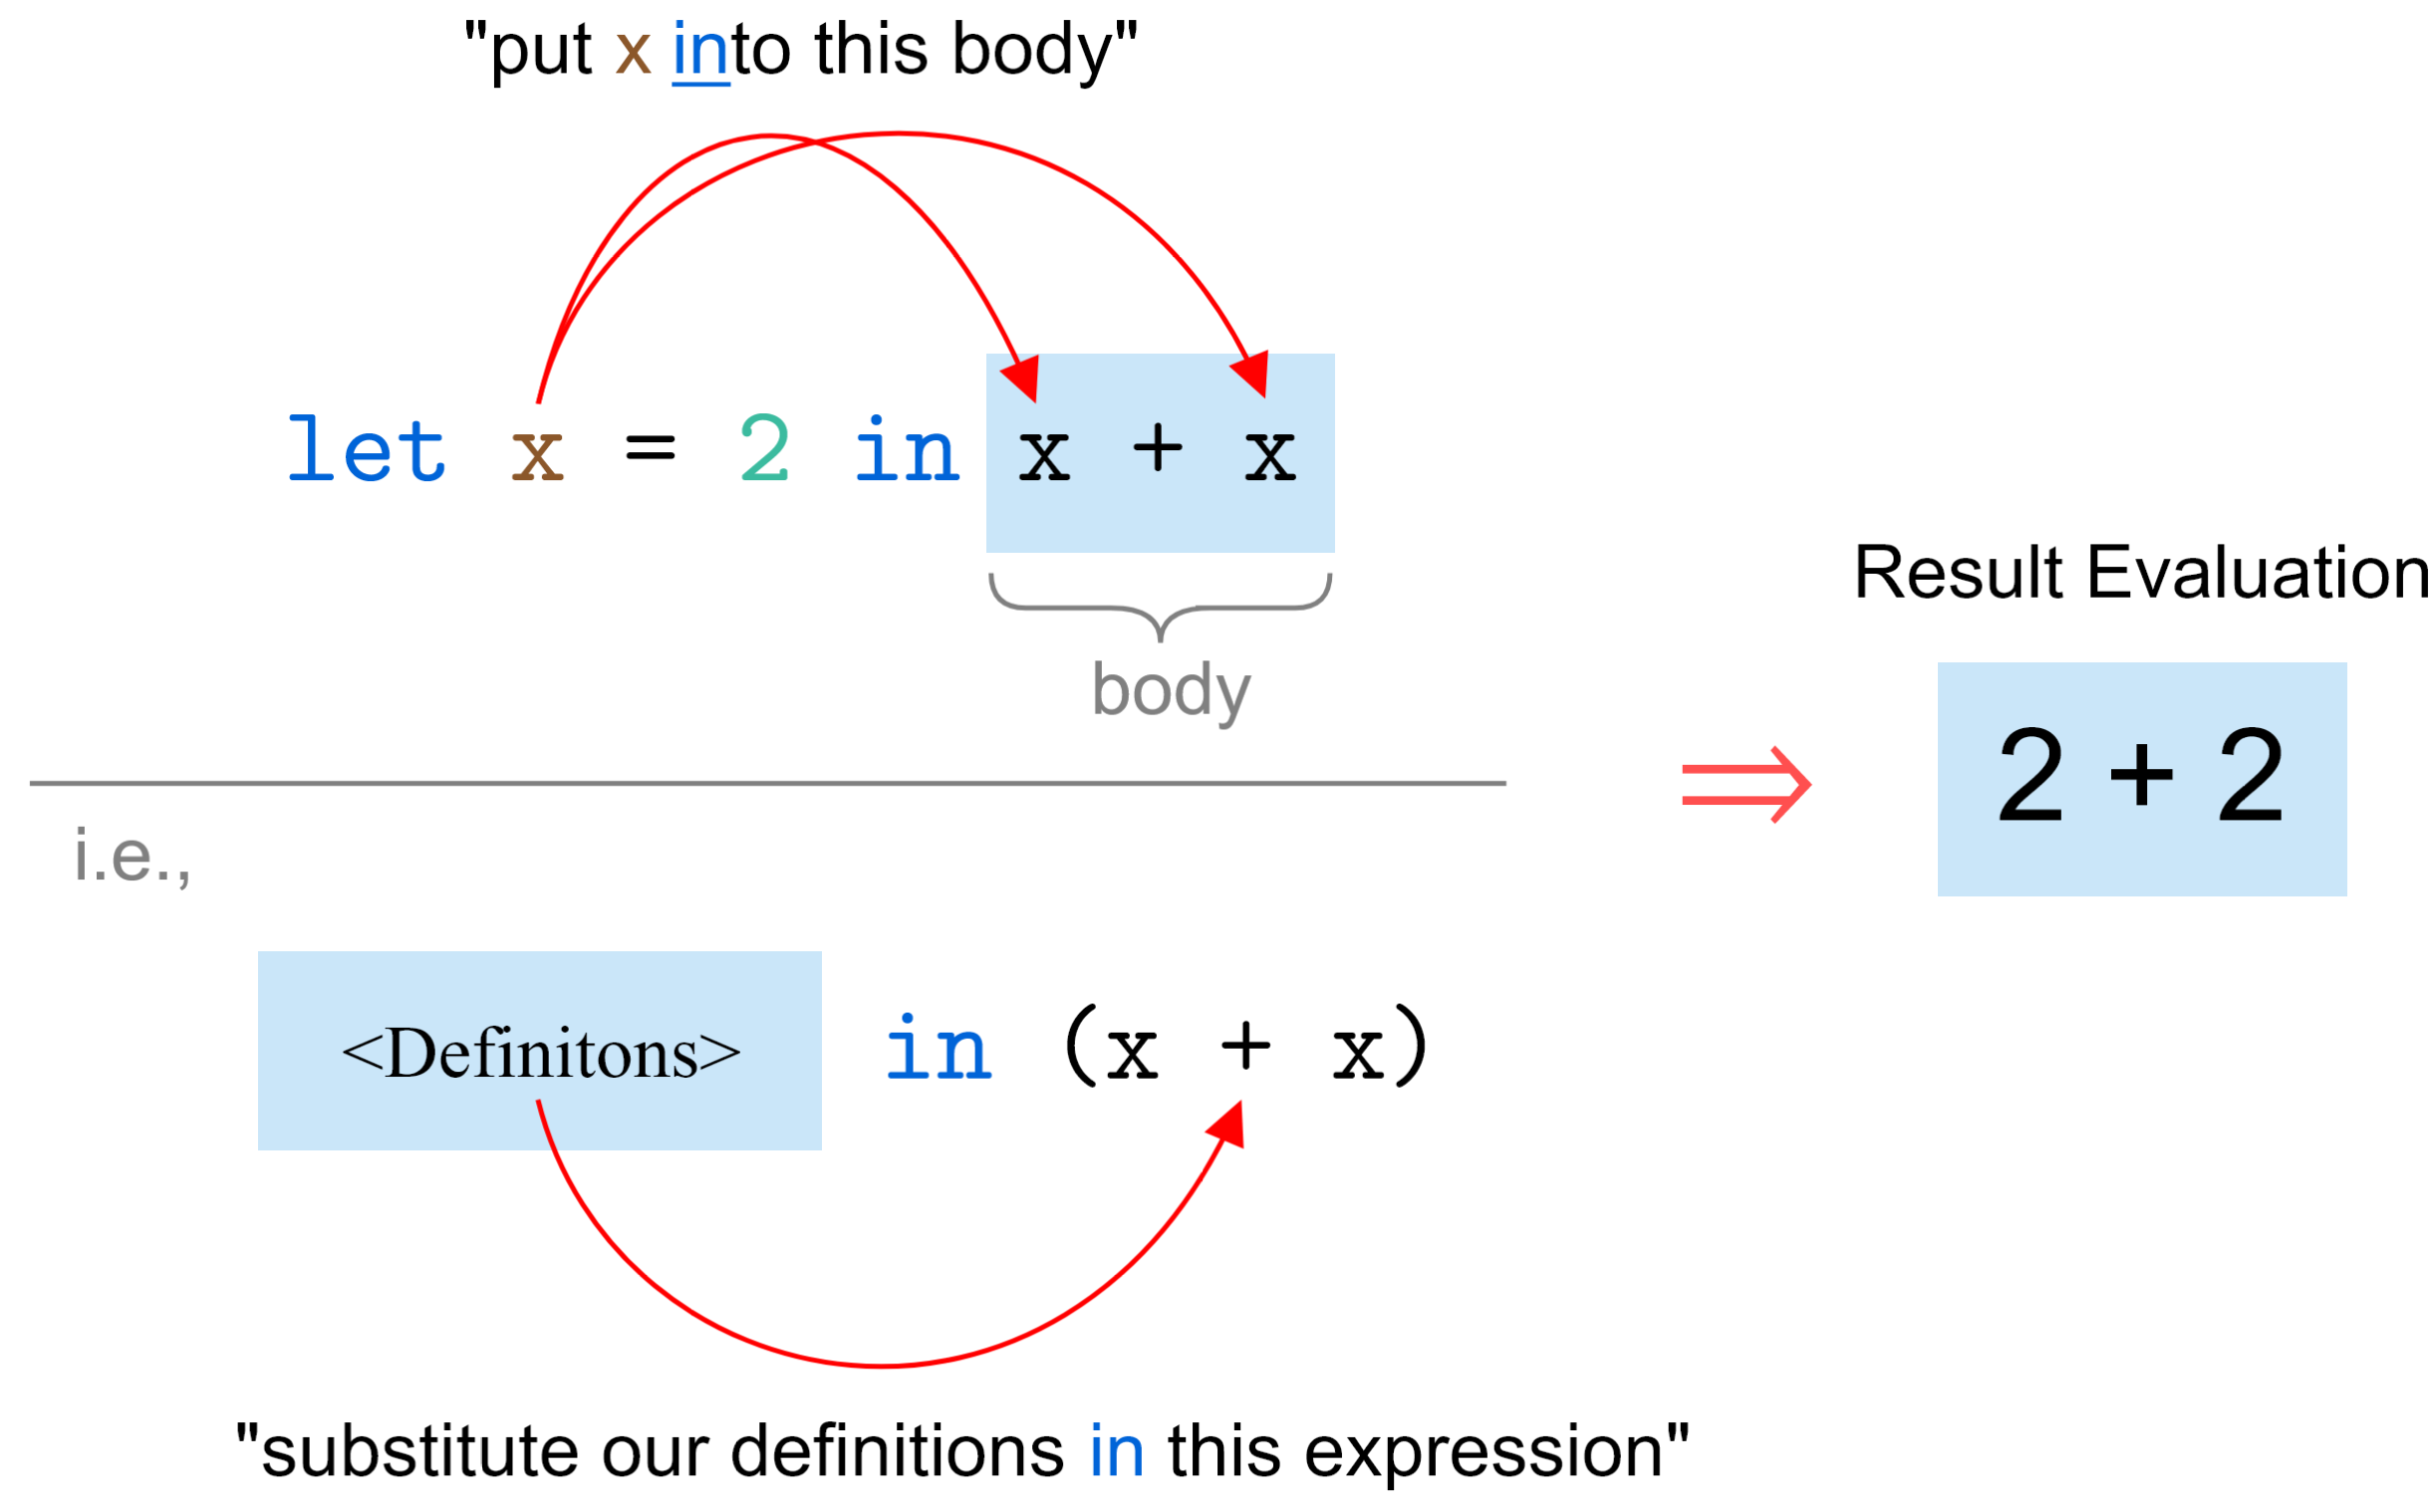
\includegraphics[width=0.8\textwidth]{Sections/Func/ocam/indef.png}\hspace{3em}}
    }
    \caption{The \snippet{in} Keyword in OCaml}
    
    \label{fig:ocaml-in}
\end{figure}



\vspace{-1em}
\noindent
To disect the roles of \textbf{syntax}, \textbf{semantics}, and \textbf{types} in the expression \snippet{let x = 2 in x + x}:

\begin{figure}[h]
    {
        \setlength{\fboxsep}{10pt}
    \centering
    \fbox{\hspace{4em} 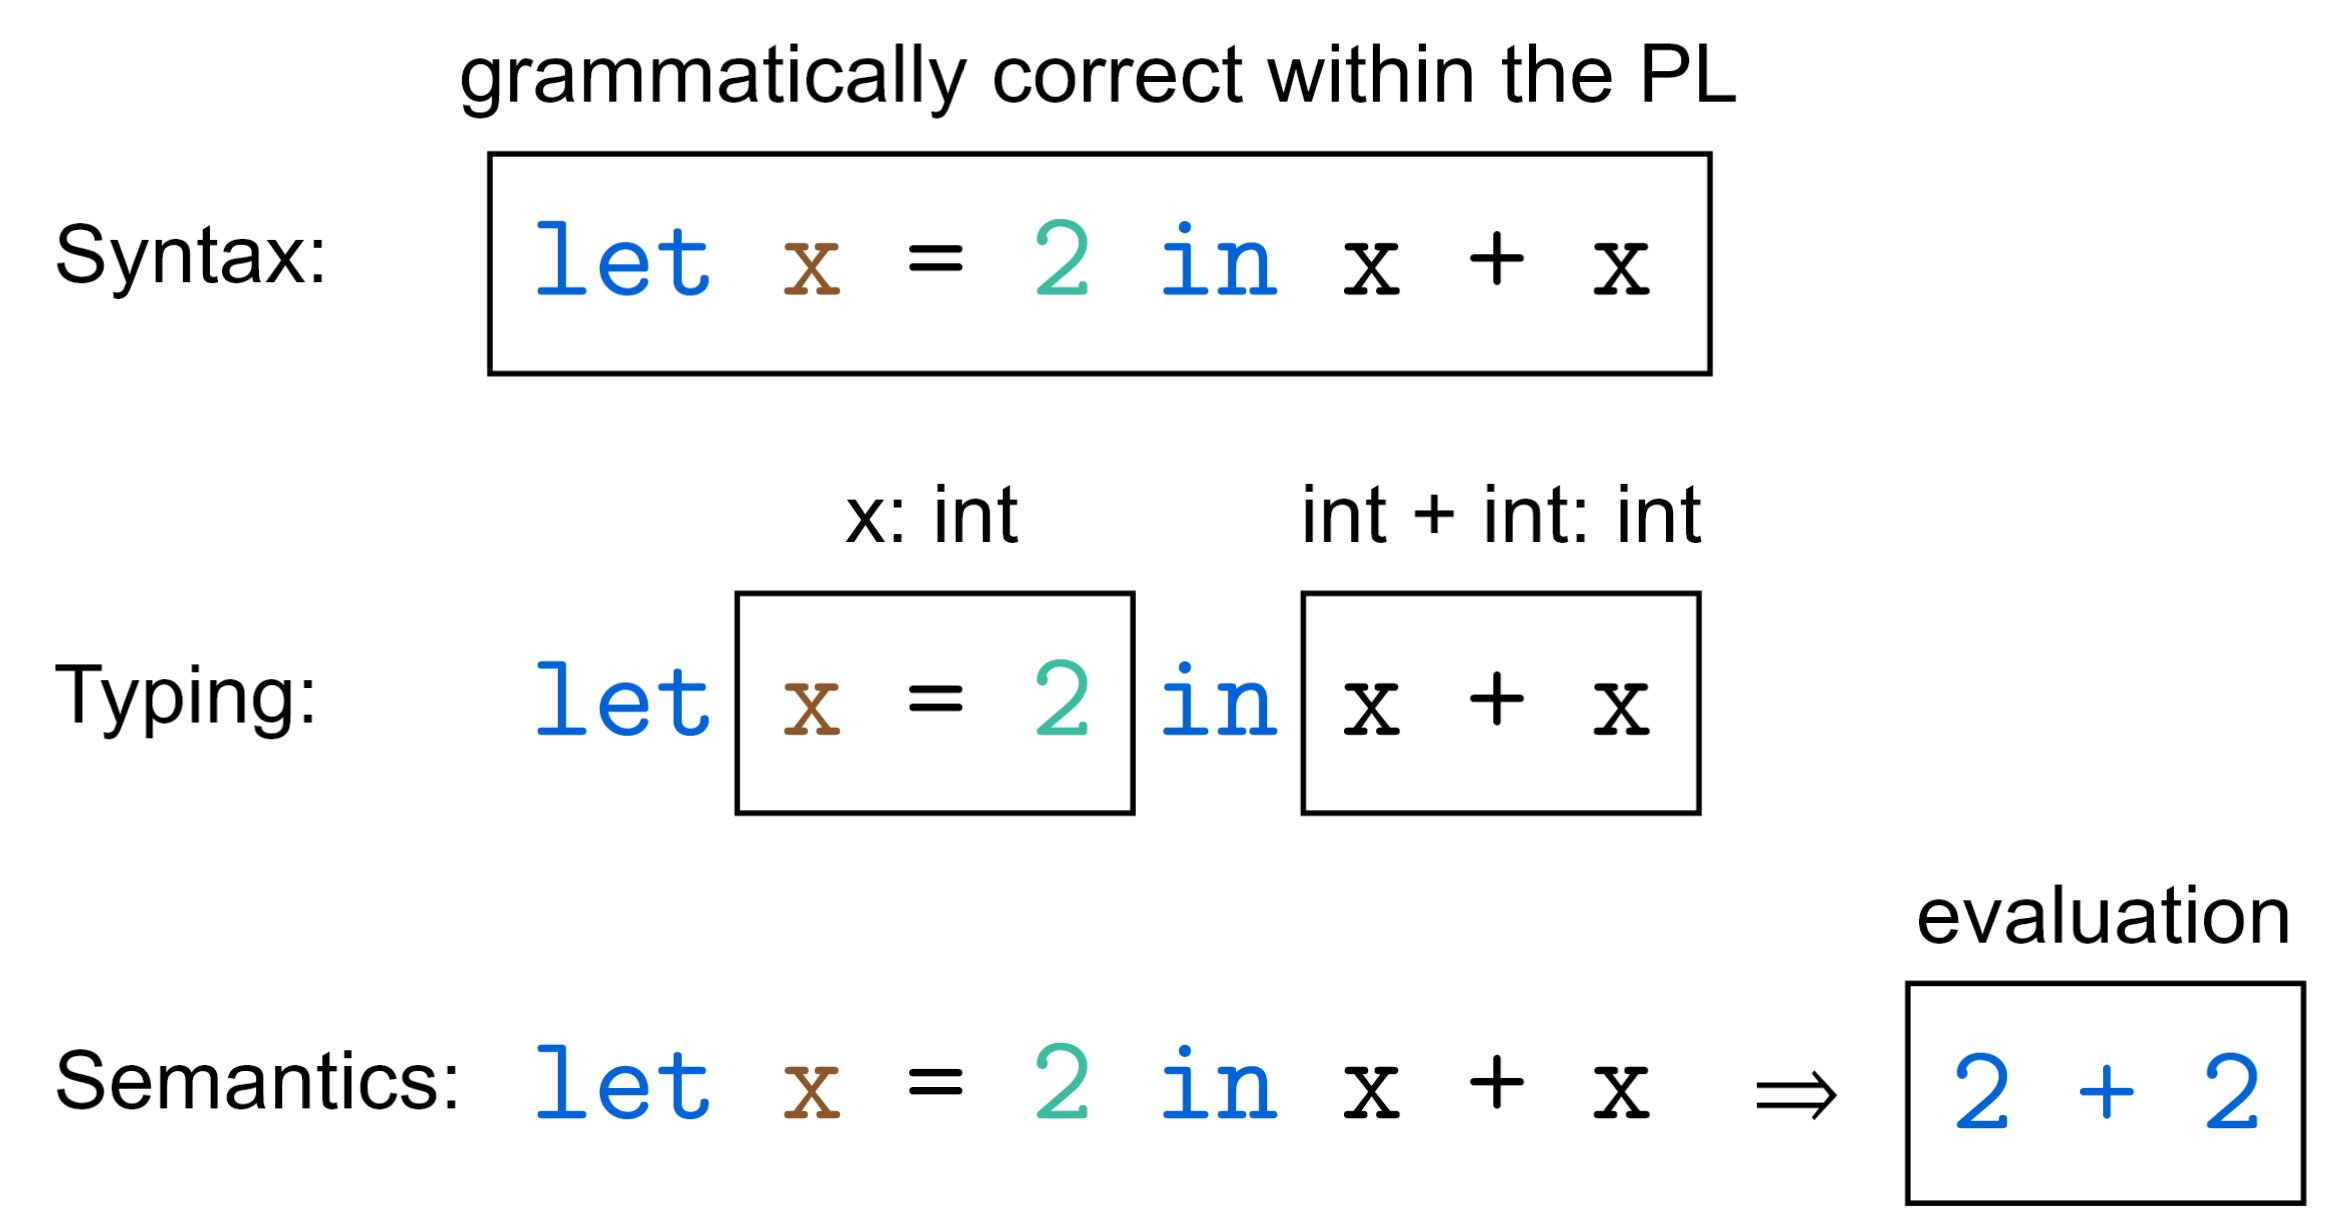
\includegraphics[width=.7\textwidth]{Sections/Func/ocam/sst.png}\hspace{5em}}
    }
    \caption{Syntax, Semantics, and Types in OCaml}
    \label{fig:ocaml-in2}
\end{figure}

\vspace{-1em}
\noindent
\begin{itemize}
    \item \textbf{Syntax}: The expression \snippet{let x = 2 in x + x} is a valid OCaml expression.
    \item \textbf{Typing}: Well-typed, as $x$ is an \snippet{int} and $x + x$ is an \snippet{int}.
    \item \textbf{Semantics}: After substitution, the expression evaluates to $2 + 2$.
\end{itemize}

\newpage 

\begin{Def}[Whitespace Agnostic]
    OCaml is \textbf{whitespace agnostic}, meaning that the interpreter does not rely on the presence or absence of whitespace to determine the structure of the code. Whitespace can be used freely for readability without affecting the semantics of the program. For example, the following expressions are equivalent:
    \begin{lstlisting}[language=OCaml, numbers=none, caption={Whitespace Agnostic Example}]
    let x = 1 + 2
    \end{lstlisting}

    and

    \begin{lstlisting}[language=OCaml, numbers=none]
    let x 
    = 1
      +
      2
    \end{lstlisting}

    \noindent
    Both produce the same result, as whitespace does not alter the meaning of the expression.
\end{Def}

\subsection{Understanding Functions in OCaml}
In OCaml, functions do not require parentheses, arguments directly follow the function name. 
For example:
\begin{lstlisting}[language=OCaml]
    let add x y z= x + y + z in 
    let result = add 3 5 5
    (* semantically evaluates to 3 + 5 + 5 *)
\end{lstlisting}

\noindent
Here, the \snippet{add} function takes two arguments, \snippet{x} and \snippet{y}, which is substituted into \snippet{result} with arguments 3,5, and 5.\\

\begin{Def}[Anonymous Functions]

An \textbf{anonymous function} is a one-time-use function that is not bound to a name. In OCaml, anonymous functions are created using the \snippet{fun} keyword.
They are useful for passing functions as arguments to other functions or for defining functions locally. For example:

\begin{lstlisting}[language=OCaml, numbers=none]
    let add x y z = x + y z
\end{lstlisting}
\noindent is equivalent to:
\begin{lstlisting}[language=OCaml, numbers=none]
    let add = fun x -> fun y -> fun z -> x + y + z
\end{lstlisting}

\noindent
These are formally known as \textbf{lambda expressions}, where in \textbf{lambda calculus} \snippet{fun x -> e} is written 
as ``$\lambda x.e$'', s.t., $\lambda$ denotes the anonymous function, $x$ the argument, and $e$ the expression.
The add function is equivalent to, $\lambda x.\lambda y.\lambda z.x + y + z$, in lambda calculus.

\end{Def}

\newpage

\noindent
Functions with multiple arguments can be thought of as nested anonymous functions, where variables are passed 
down the chain of functions. To illustrate:

\begin{figure}[h]
    {
    \setlength{\fboxsep}{16pt}
    \centering
    \fbox{\hspace{2em}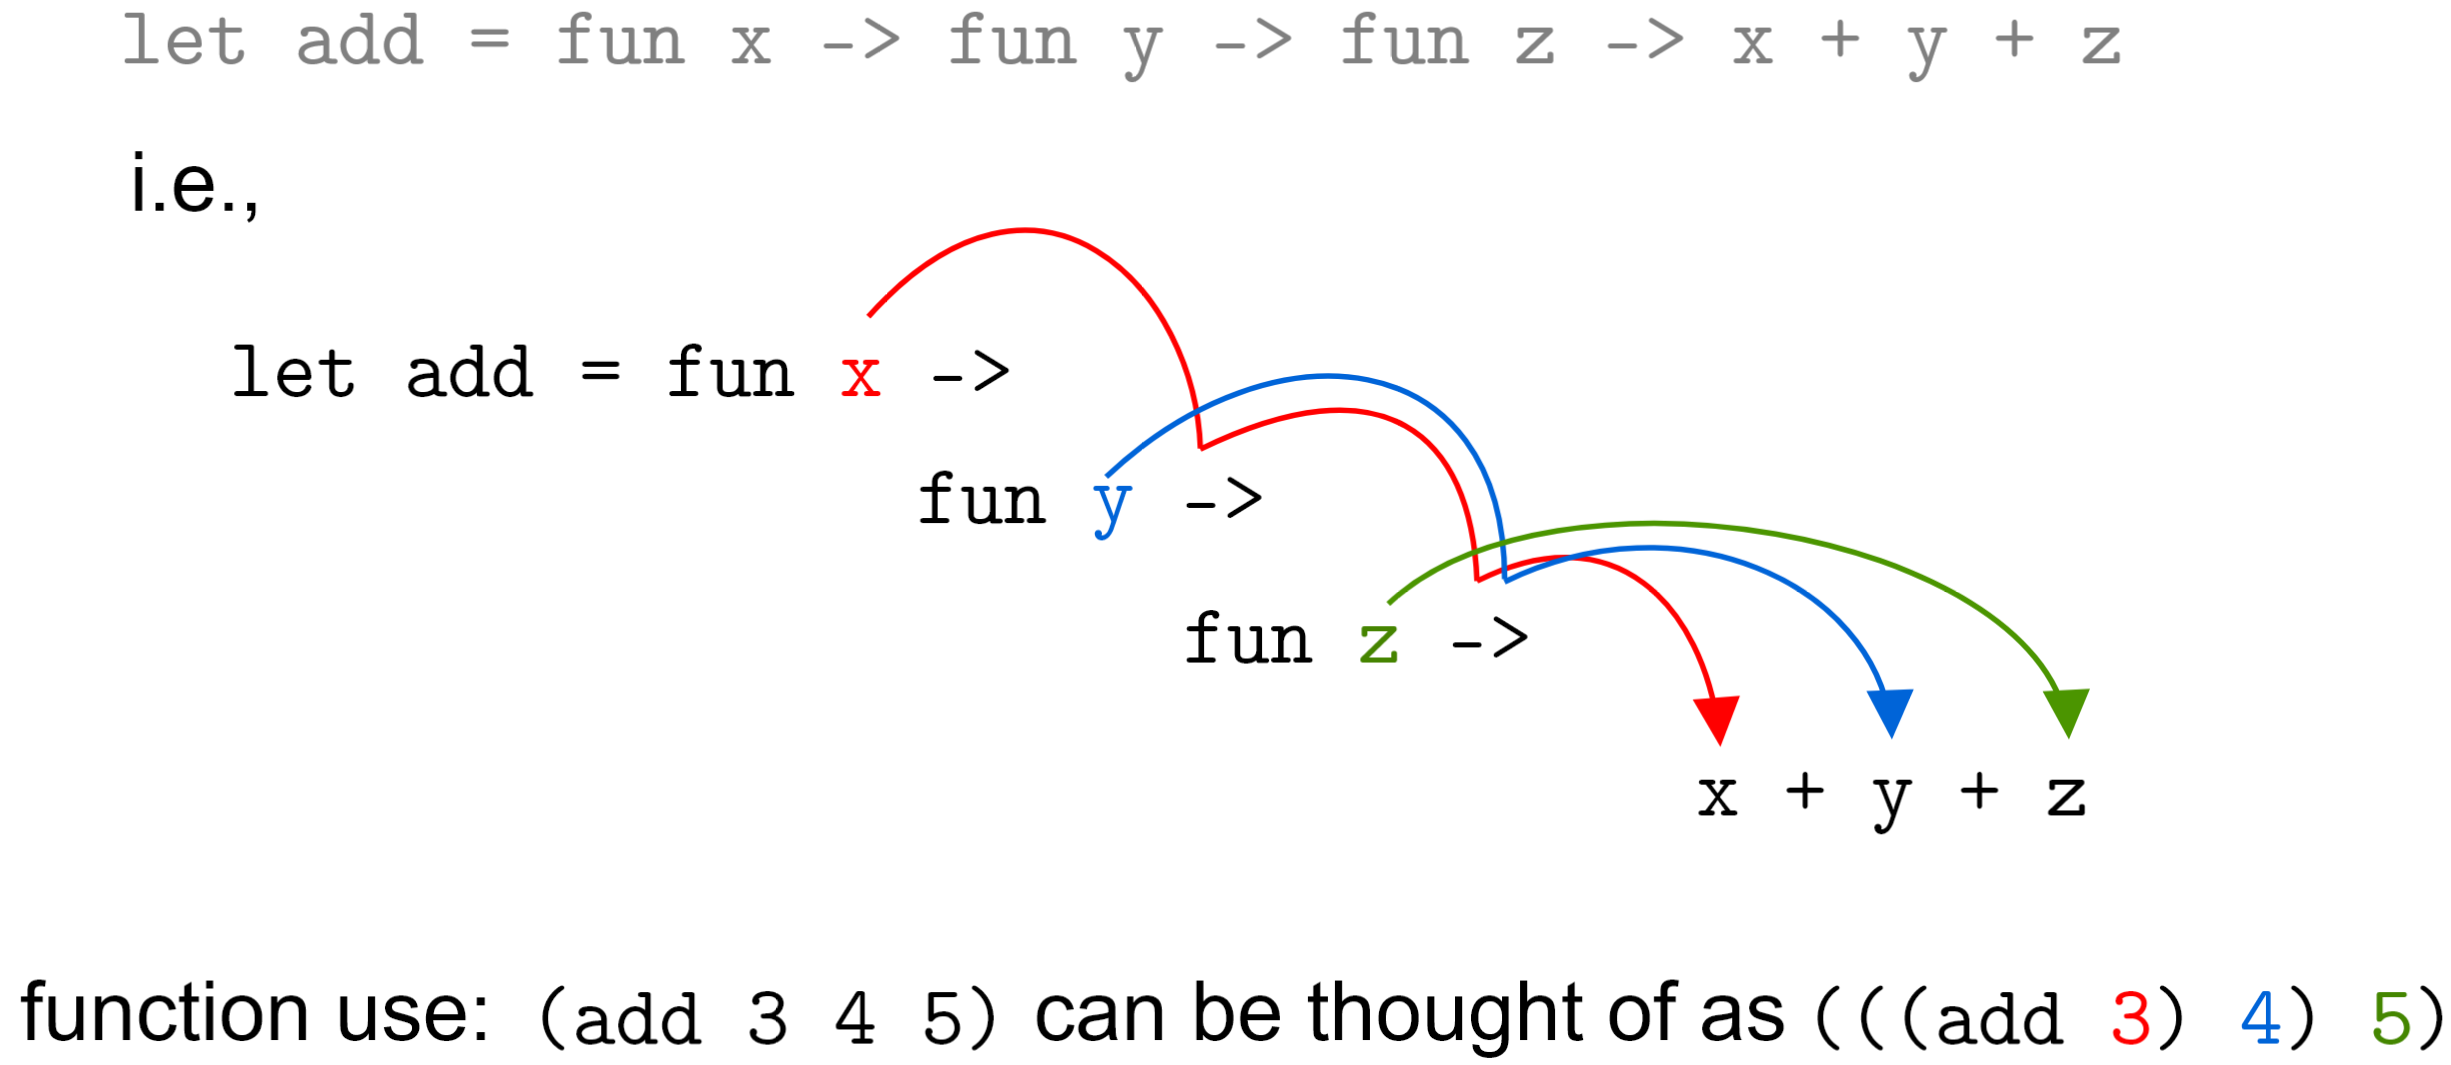
\includegraphics[width=0.8\textwidth]{Sections/Func/ocam/curry.png}\hspace{3em}}
    }
    \caption{Anonymous Functions in OCaml}
    
    \label{fig:ocaml-anon}
\end{figure}

\vspace{-1em}
\noindent
Alternatively, we may illustrate an analogous example with scoped functions in a pseudo syntax:

\begin{figure}[h]
    {
    \setlength{\fboxsep}{0pt}
    \centering
    \fbox{\hspace{8.7em}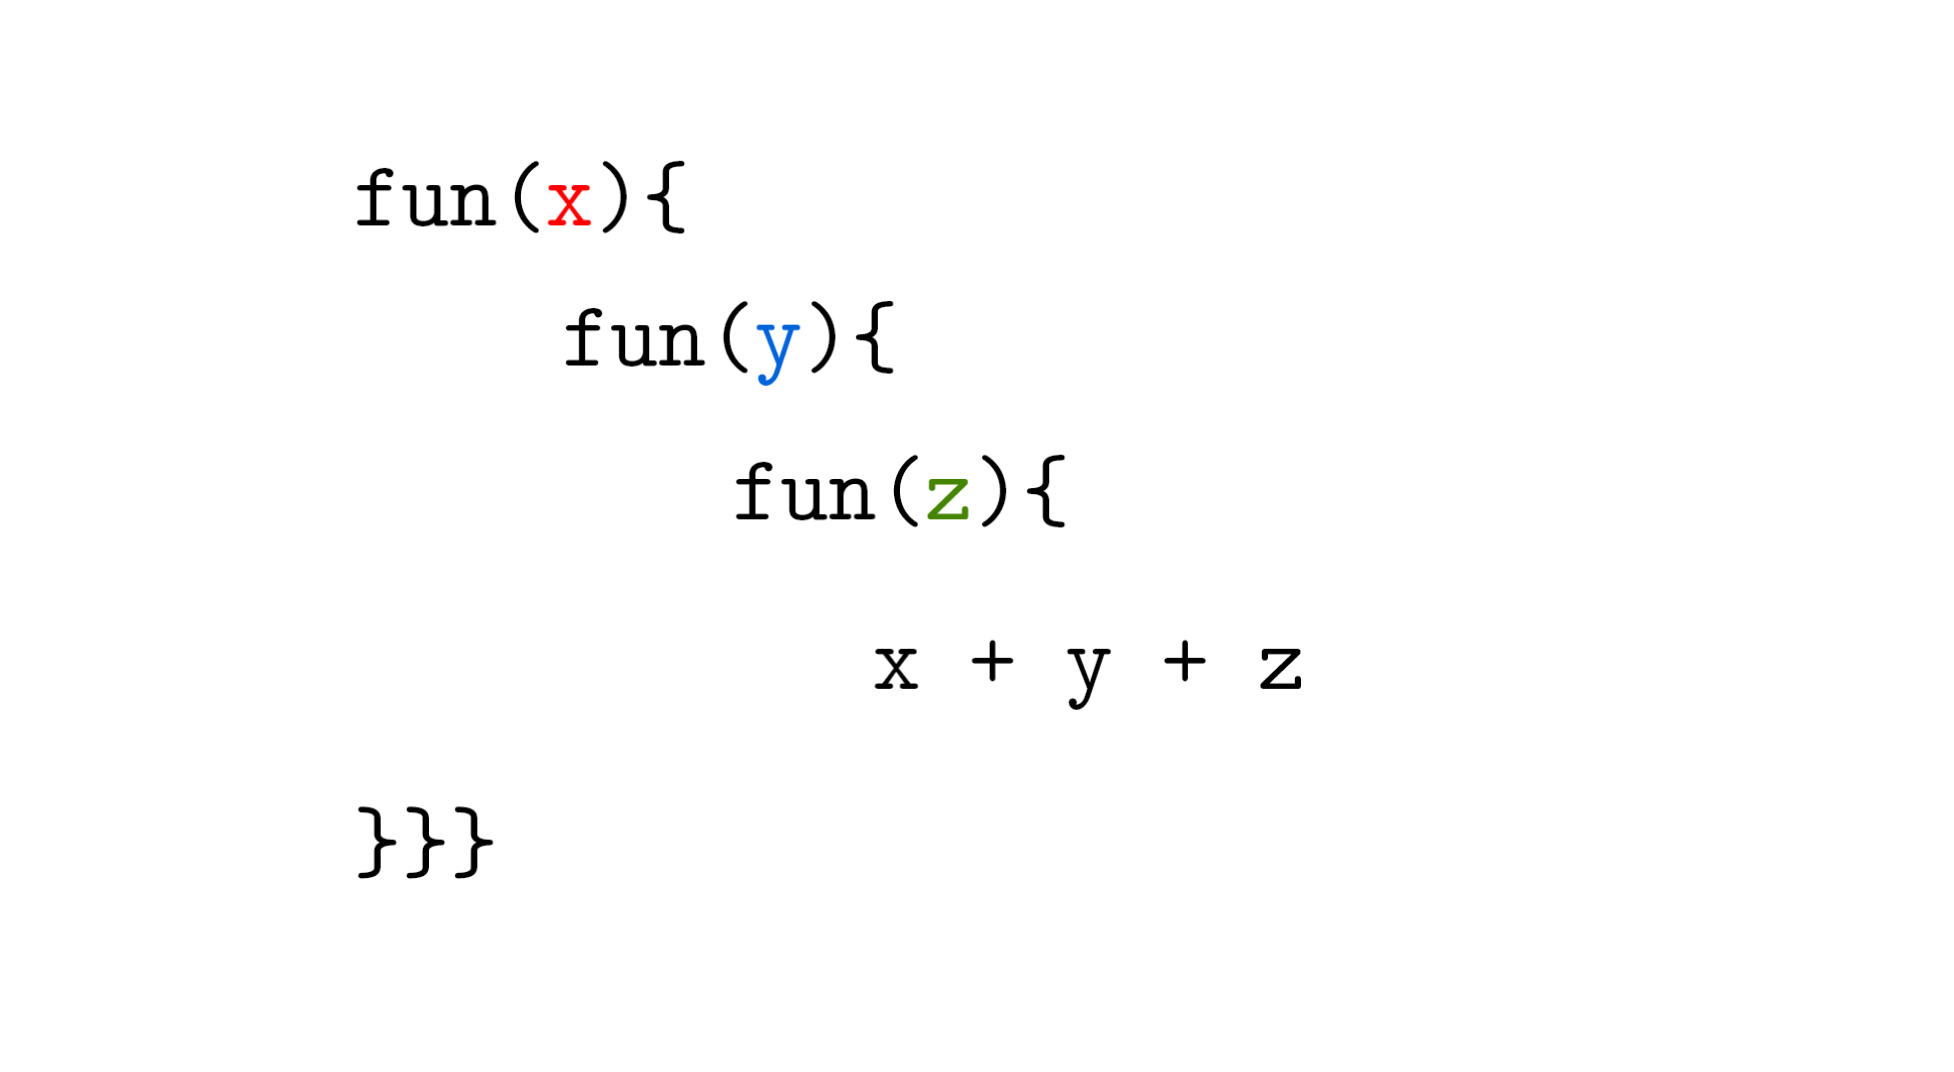
\includegraphics[width=0.6\textwidth]{Sections/Func/ocam/curry2.png}\hspace{8em}}
    }
    \caption{Anonymous Functions in OCaml}
    
    \label{fig:ocaml-anon2}
\end{figure}

\vspace{-.5em}
\noindent
Where $x$ is a local variable of the outer-most function within scope of the inner functions, and so on with $y$ and $z$.
This is the concept known as \textbf{currying}.

\begin{Tip}
    Lambda calculus was developed by \textbf{Alonzo Church} in the 1930s at Princeton University. Church was the doctoral advisor of \textbf{Alan Turing}, the creator of the Turing Machine (1936), a theoretical model that laid the groundwork for modern computation.
    
    Curry functions were introduced by \textbf{Haskell Curry} around the 1940-1950s as he worked in the U.S. He expanded upon combinatory logic, emphasizing breaking down functions into a sequence of single-argument functions.
\end{Tip}
    

\newpage

\begin{Def}[Curried Functions]

A \textbf{curried function} is a function that, when applied to some arguments, returns another function that takes the remaining arguments. For example:
\[
\texttt{add x y = x + y}
\]
is internally equivalent to:
\[
\texttt{add = fun x -> (fun y -> x + y)}
\]

In OCaml, functions are \textbf{curried} by default. This means that a function of multiple arguments is treated as a sequence of single-argument functions.
\end{Def}

\vspace{1em}
\noindent
We let \snippet{add} stand for \snippet{fun x -> fun y -> x + y}. Therefore in reality we are doing:
\begin{lstlisting}[language=OCaml, numbers=none]
    (fun x -> fun y -> x + y) 3 5
\end{lstlisting}

\noindent
This is know as \textbf{Application}, as we are \textit{applying} arguments to a function.

\vspace{1em}
\begin{Def}[Application]

    \textbf{Application} is the process of applying arguments to a function. \textbf{Full application} is when all 
    arguments are applied to a function. For example:

    \begin{lstlisting}[language=OCaml, numbers=none]
        (fun x -> fun y -> x + y) 3 5
    \end{lstlisting}

    \noindent
    Here, the function \snippet{fun x -> fun y -> x + y} is fully applied to the arguments 3 and 5.\\

    \noindent
    \textbf{Partial application} is when only some arguments are applied to a function, which evaluates to another function 
    accepting the remaining arguments. For example:

    \begin{lstlisting}[language=OCaml, numbers=none]
        (fun x -> fun y -> x + y) 3
    \end{lstlisting}

    \noindent
    Here, the function \snippet{fun x -> fun y -> x + y} is partially applied to the argument 3, resulting in a new function
    \snippet{fun y -> 3 + y}.\\

    \noindent
    \textbf{In Lambda Calculus} we may represent this as:
    \begin{align*}
        (\lambda x. \lambda y. (x + y))&\ 3\ 5 \rightarrow\\
        (\lambda y. (3 + y))&\ 5 \rightarrow\\
        (3 + 5) \hspace{.4em} &
    \end{align*}
    In this process, arguments are sequentially applied to the corresponding variables.
\end{Def}

\noindent


\newpage
\subsection{If-Expressions}
In OCaml, \textbf{if-expressions} are used to conditionally evaluate expressions. This behaves similarly to other PLs with a few distinctions.

\begin{Def}[Ocaml if-then-else]

    In OCaml, if statements follow the form: \snippet{if <condition> then <expr1> else <expr2>}, i.e., 
    if the condition is true, then \snippet{expr1} is evaluated, else \snippet{expr2} is evaluated. For example:
    \begin{lstlisting}[language=OCaml, caption={If-Expression: Divisible by 2}, numbers=none]
        fun x -> if x mod 2 = 0 then "even" else "odd"
    \end{lstlisting}

    \noindent
    Here, the anonymous function finds if $x$ is divisible by 2, evaluating to \snippet{"even"} if true, or otherwise \snippet{"odd"}.

    \noindent
    \rule{\textwidth}{0.4pt}

    \vspace{.3em}
    \noindent
    \textbf{Typing}: The \snippet{then} and \snippet{else} expressions must evaluate to the same type. 
    So the following expression is \textbf{invalid}:

    \begin{lstlisting}[language=OCaml, caption={Invalid If-Expression}, numbers=none]
        fun x -> if x mod 2 = 0 then "even" else 0 (* INVALID *)
    \end{lstlisting}

    \noindent
    \rule{\textwidth}{0.4pt}

    \vspace{.3em}
    \noindent
    \textbf{Else If}: In OCaml, there is no \snippet{else if} keyword. Instead, nested if-expressions are used to achieve the same effect.

    \begin{lstlisting}[language=OCaml, caption={Else If Example}, numbers=none]
        fun x -> 
            if x mod 3 = 0 then 
                "divisible by 3"
            else if x mod 5 = 0 then
                "divisible by 5" 
            else "not divisible by 2 or 3"
    \end{lstlisting}
\end{Def}

\begin{Q




        